\documentclass[spanish]{article}

\usepackage{mystyle}
\usepackage{myvars}
\usepackage{mylinearprogramming}



%-----------------------------

\begin{document}

	\maketitle % Insert title

	\thispagestyle{fancy} % All pages have headers and footers


%-----------------------------
%	ABSTRACT
%-----------------------------

	\begin{abstract}
		\noindent Problemas de Localización de servicios \url{https://github.com/garciparedes/mosel-examples/tree/master/service-location-examples}\cite{garciparedes:mosel-examples}
	\end{abstract}

%-----------------------------
%	TEXT
%-----------------------------


  \section{Set Covering Problem: Distancias}
	\label{sec:1}

    \paragraph{}
		El problema de \emph{set convering} o \emph{cubrimiento de conjuntos} consiste en la asignación de un conjunto de recursos $n$ recursos $x_{j}$ cuyo uso tiene un coste de $c_{j}$ para cumplir $m$ necesidades. Las necesidades que cubre cada recurso se representan a través de $a_{ij}$. La modelización matemática de este problema se muestra en la ecuación \eqref{eq:set_covering}.


		\begin{eqfloat}
			\begin{equation}
				\begin{array}{ll@{}ll}
					\text{Minimizar}	& \displaystyle\sum\limits_{j=1}^{n} c_{j}	&	x_{j} &\\
					\text{sujeto a}		& \displaystyle\sum\limits_{j = 1}^n a_{ij}	&	x_{j} \geq 1,  &i=1 ,..., m\\
													 	&                                           &	x_{j} \in \{0,1\}, &j=1 ,..., n
				\end{array}
			\end{equation}
      \caption{Formulación del Problema de Cubrimiento Total.}
      \label{eq:set_covering}
    \end{eqfloat}

		\subsection{Distancia de cubrimiento inferior a 50km}
		\label{sec:1.1}

			\paragraph{}
			En este caso se ha propuesto resolver el problema de cubrimiento máximo para la asignación de los lugares donde situar los puntos de servicio de entre 30 ciudades (por tanto $m = n = 30$) para poder abastecer a todos ellos en una distancia inferior a 50 km. Puesto que todos los recursos presentan el mismo coste, en este caso $\forall j \ c_{j} = 1$.

			\paragraph{}
			La solución a este problema se muestra en la ecuación \eqref{eq:sol-1.1}, la cual requiere de \textbf{18} recursos

			\begin{equation}
			\label{eq:sol-1.1}
				x_{j} =
					\begin{cases}
		      	1 & j \in S = \{2,  4,  5,  9,  10,  11,  12,  13,  14,  16,  17,  18,  21,  22,  27,  28,  29,  30 \} \\
		      	0 & otherwise
			   	\end{cases}
			\end{equation}

		\subsection{Distancia de cubrimiento desde 1 a 250km}
		\label{sec:1.2}

			\paragraph{}
			En este caso, se ha resuelto el mismo problema que en el apartado anterior, pero esta vez de manera iterativa conforme a las distancias necesarias mínimas de cubrimiento en el intervalo $dc \in [1, 250]$. Dichos resultados se muestran en la figura \ref{fig:sol-1.2}. Los resultados completos de todas las iteracciones pueden obtenerse ejecutando el correspondiente fichero mosel\cite{garciparedes:mosel-examples} y examinando el fichero CSV resultante.

			\begin{figure}[h]
				\begin{center}
					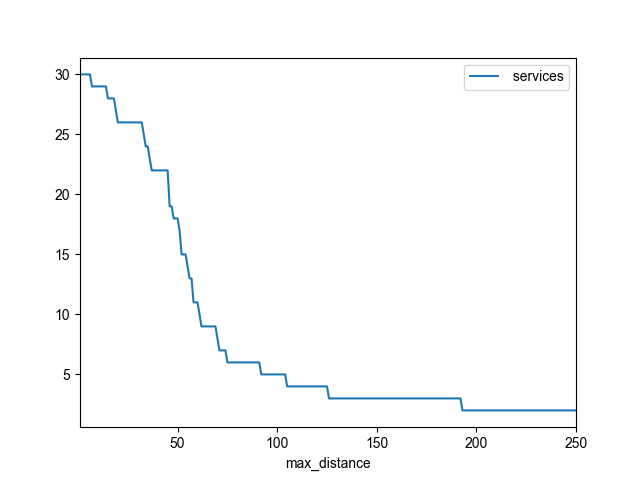
\includegraphics[width=0.7\textwidth]{tema-2-p1-output}
				\end{center}
				\caption{Relación entre la distancia mínima de para que una ciudad se considere cubierta y el número de recursos necesarios para dicha tarea.}
				\label{fig:sol-1.2}
			\end{figure}

	\section{Set Covering Problem: Datos dispersos}
	\label{sec:2}

    \paragraph{}
		En este caso, el problema posee las mismas características que el descrito en la sección \ref{sec:1}, cuya modelización matemática se muestra en la ecuación \eqref{eq:set_covering}. Sin embargo, la novedad que tiene este respecto del anterior es que en este caso los datos son suministrados en forma una matriz dispersa, lo que reduce el tamaño del fichero de datos por lo que se prescinde de las entradas cuyo valor es $0$.

		\subsection{Localización de centros de Ambulancias}
		\label{sec:2.1}

			\paragraph{}
			En este caso se pide resolver el problema de cubrir $m = 20$ distritos a partir de $n = 10$ centros de ambulancias. Para conocer en qué distritos son cubiertos por qué puntos de servicio se suministra además la matriz dispersa $a$ codificada tal y como se infica en la \eqref{eq:binary-encoding}. Tal y como ocurre en el apartado anterior, los costes también son constantes por lo que $\forall j \ c_{j} = 1$

			\begin{equation}
			\label{eq:binary-encoding}
				a_{ij}  =
					\begin{cases}
		      	1 & \text{El distrito i es cubierto por el centro de ambulancias j}\\
		      	0 & otherwise
			   	\end{cases}
			\end{equation}

			\paragraph{}
			Los puntos de asignación óptimos para este problema se muestran en la ecuación \eqref{eq:sol-2.1}, es decir, para cubrir las necesidades de todos los distritos se han de colocar $6$ centros de ambulancias.

			\begin{equation}
			\label{eq:sol-2.1}
				x_{j} =
					\begin{cases}
		      	1 & j \in S = \{2,  3,  4,  6,  8,  10 \} \\
		      	0 & otherwise
			   	\end{cases}
			\end{equation}


		\subsection{Planificación de Viajes en Empresa de aviación American Airlines}
		\label{sec:2.2}

			\paragraph{}
			Este problema se basa en la planificación acerca de la tripulación de una empresa de aviación, de tal manera que se aproveche lo más posible la jornada labolar de sus trabajadores. En este caso, se trata de planificar la tripulación que formará parte de $m = 12$ vuelos, que se compone de un total de $n = 15$ trabajadores. En este caso la codificación de la matriz $a$ sigue la misma distribución qu el ejercicio \ref{sec:2.1}, por lo que la descripción de la ecuación \eqref{eq:binary-encoding} sigue siendo válida. La principal novedad con respecto a los casos anteriores es que el vector de costes $c_j$ en este caso ya no toma el valor unidad, sino que se refiere al sueldo de cada uno de los trabajadores, es decir, $c_j = \text{Sueldo del trabajador j}$.

			\paragraph{}
			La asignación óptima se muestra en la ecuación \eqref{eq:sol-2.2} y presenta un coste total de $9100 = 2900 + 2600 + 3600$.

			\begin{equation}
			\label{eq:sol-2.2}
				x_{j} =
					\begin{cases}
		      	1 & j \in S = \{ 1, 9, 12  \} \\
		      	0 & otherwise
			   	\end{cases}
			\end{equation}


	\section{Set Covering Problem: Sayre-Priors}
	\label{sec:3}

		\paragraph{}
		El ejercicio de \emph{Sayre-Priors} presenta el mismo planteamiento que el anterior del apartado \ref{sec:2.2}, por tanto la descripción que se ha realizado en el anterior caso es válida para este. Los únicos cambios son los datos de entrada, que en este caso tienen la siguiente dimensionalidad: Se debe encontrar el resultado óptimo para $m = 10$ vuelos y una tripulación de $n = 37$ trabajadores.

		\paragraph{}
		La asignación óptima se muestra en la ecuación \eqref{eq:sol-3} y genera un coste de $2 + 2 + 3 + 3 = 10 $ mil dolares.

\begin{equation}
		\label{eq:sol-3}
			x_{j} =
				\begin{cases}
					1 & j \in S = \{ 12, 24, 29, 32  \} \\
					0 & otherwise
				\end{cases}
		\end{equation}


	\section{Max Covering Problem}
	\label{sec:4}

		\paragraph{}
		En esta sección se trata el \emph{problema de cubrimiento máximo} o \emph{max covering problem}. El problema consiste en lo siguiente: Sea $m$ el número de puntos de demandas y $n$ el de puntos de servicio. El objetivo se trata de maximizar el beneficio $h_i$ obtenido de cubrir el í-esimo punto de demanda. Para modelizar dicho cubrimiento se utiliza la variable binaria $z_i$. Para representar los puntos de servicio utilizados se utiliza la variable de tipo binario $x_j$. La motivación del problema consiste en encontrar el conjunto de variables $x_j$ con cardinalidad máxima denominada por $p$ y prefijada previamente, que máximize la ganancia debida al cubrimiento de los puntos de servicio $z_i$.

		\begin{eqfloat}
			\begin{equation}
				\begin{array}{ll@{}ll}
					\text{Maximizar}
						& \displaystyle\sum\limits_{i = 1}^{m} h_{i} & z_{i} 			&							\\
					\text{sujeto a}
						& \displaystyle\sum\limits_{j \in N_i}& x_{j} \geq z_i,		&i=1 ,..., m	\\
						& \displaystyle\sum\limits_{j = 1}^n 	& x_{j} \leq p,  		& 						\\
						&                                     &	x_{j} \in \{0,1\},&j=1 ,..., n 	\\
						&                                     &	z_{i} \in \{0,1\},&i=1 ,..., m  \\
				\end{array}
			\end{equation}
			\caption{Formulación del Problema de Cubrimiento Máximo.}
      \label{eq:max_covering}
    \end{eqfloat}

			\paragraph{}
			En esta sección se proponen tres ejercicios para resolver este problema, los cuales han sido resueltos para distintos valores de $p$.

		\subsection{Usuarios Alcanzados a partir de anuncios en $p$ Revistas}
		\label{sec:4.1}

			\paragraph{}
			En este problema se trata de encontrar el máximo número de personas cubiertas a partir de la publicación de anunciós en revistas. Los datos de entrada están formados por $n = 10$ revistas que pueden ser alcanzadas por $m = 50$  personas. Para ello se proporciona la matriz $a$ de carácter binario representando la posición $a_{ij}$ que la revista $j$ es leida por la persona $i$. Se pide resolver el problema para los valores de $p = [1, 10] \in N$. Los resultados se muestran en la tabla \ref{table:sol-4.1}.

			\begin{table}[h]
				\begin{center}
					\begin{tabular}{|c || c || l |}
						\hline
						$p$		&	\% Cubierto	& Puntos Abiertos \\ \hline \hline
						$1$ 	& $32\%$ & $\{5\}$ \\ \hline
		     		$2$ 	& $48\%$ & $\{5, 6\}$ \\ \hline
						$3$ 	& $64\%$ & $\{2,3,5\}$ \\ \hline
						$4$ 	& $76\%$ & $\{3,5,6,7\}$ \\ \hline
						$5$ 	& $84\%$ & $\{3,5,6,7,8\}$ \\ \hline
						$6$ 	& $90\%$ & $\{1,3,5,6,7,8\}$ \\ \hline
						$7$ 	& $94\%$ & $\{1,3,5,6,7,8,10\}$ \\ \hline
						$8$ 	& $96\%$ & $\{1,3,4,5,6,7,8,10\}$ \\ \hline
						$9$ 	& $98\%$ & $\{1,3,4,5,6,7,8,9,10 \}$ \\ \hline
						$10$	& $98\%$ & $\{1,2,3,4,5,6,7,8,9,10\}$ \\
						\hline
					\end{tabular}
				\end{center}
				\caption{Resultados del ejercicio \ref{sec:4}.\ref{sec:4.1}.}
				\label{table:sol-4.1}
			\end{table}


		\subsection{Zonas Cubiertas a partir de $p$ de centros de Ambulancias}
		\label{sec:4.2}

			\paragraph{}
			En este ejercicio se pide resolver el problema de máximo cubrimiento para los valores de $p = [1, 10] \in N$ al igual que en la sección anterior. En este caso el problema se refiere al cubrimiento de $m = 20$ zonas geográficas a partir de $n=10$ ambulancias, por tanto se trata de encontrar el máximo número de zonas cubiertas con la utilización de $p$ ambulancias.

			\paragraph{}
			En este caso, además de la matriz $a$ que codifica de manera binaria en $a_{ij}$ que la zona $i$ es cubierta por la variable $j$, se proporciona el vector $h$, que representa en la componente $h_i$ el beneficio obtenido por cubrir la zona $i$. Esto podría interpretarse como el número de personas que se abarcan en dicha zona.

			\paragraph{}
			Los resultados de en este caso se muestran en la tabla \ref{table:sol-4.2}. Tras analizar los resultados obtenidos se puede obtener como conclusión que el valor óptimo es $p = 6$, es decir, con la utilización de 6 ambulancias se cubren las 20 zonas.


			\begin{table}[h]
				\begin{center}
					\begin{tabular}{|c || c || l || c | }
						\hline
						$p$		&	\% Cubierto	& Puntos Abiertos 					& f.objetivo \\ \hline \hline
						$1$ 	& $44.18\%$ & $\{4\}$ 										& $115.8$ \\ \hline
		     		$2$ 	& $63.94\%$ & $\{4, 6\}$									& $156.9$ \\ \hline
						$3$ 	& $77.59\%$ & $\{4,5,9\}$ 								& $190.4$ \\ \hline
						$4$ 	& $83.63\%$ & $\{3,4,5,9\}$ 							& $212.6$ \\ \hline
						$5$ 	& $93.76\%$ & $\{3,4,6,8,10\}$ 						& $230.4$ \\ \hline
						$6$ 	& $100\%$ 	& $\{2,3,4,6,8,10\}$					& $245.4$ \\ \hline
						$7$ 	& $100\%$ 	& $\{1,2,3,5,6,8,10 \}$				& $245.4$ \\ \hline
						$8$ 	& $100\%$ 	& $\{1,2,3,4,5,6,8,10\}$			& $245.4$ \\ \hline
						$9$ 	& $100\%$ 	& $\{2,3,4,5,6,7,8,9,10\}$ 		& $245.4$ \\ \hline
						$10$	& $100\%$ 	& $\{1,2,3,4,5,6,7,8,9,10\}$	& $245.4$ \\
						\hline
					\end{tabular}
				\end{center}
				\caption{Resultados del ejercicio \ref{sec:4}.\ref{sec:4.2}.}
				\label{table:sol-4.2}
			\end{table}


		\subsection{Zonas Cubiertas a partir de $p$ centros de Servicio Sanitario}
		\label{sec:4.3}

			\paragraph{}
			Este ejercicio se refiere a la resolución dos problemas de cubrimiento máximo de gran tamaño. Se pide resolver para los valores de $p = [1, 10] \in N$ en ambos casos. Debido al tamaño del problema, en este caso se considera que una zona de demanda $i$ ha sido cubierta si existe una zona de servicio $j$ a una distancia $dc \leq 250$ kilómetros. Al igual que en el caso anterior, también se proporciona un vector $h$, que en la posición $h_i$ representa la demanda en la zona $i$. El objetivo a maximizar por tanto es la demanda cubierta total. En este caso, la matriz $a$ no es de carácter binario, sino que se compone de atributos reales, positivos, almacenando la posición $a_{ij}$ la distancia en hectómetros de la zona de demanda $i$ al punto de servicio $j$. Por lo tanto, para utilizar la misma unidad de medida para todas las variables, se transforma la variable $dc = 250 * 10 = 2500$ hectómetros.

			\paragraph{}
			[TODO terminar ejercicio con NEOS server]

			\paragraph{}
			En el caso del primer fichero de datos de entrada denominado \textbf{aint1.dat} se recogen un total de $m = 356$ puntos de demanda y $n=22$ puntos de servicio. La solución para los distintos valores de $p$ se recogen en la tabla \ref{table:sol-4.3a}.

			\begin{table}[h]
				\begin{center}
					\begin{tabular}{|c || c || l || c | }
						\hline
						$p$		&	\% Cubierto	& Puntos Abiertos 					& f.objetivo \\ \hline \hline
						$1$ 	& $0\%$ & $\{\}$ 										& $0$ \\ \hline
						$2$ 	& $0\%$ & $\{\}$ 										& $0$ \\ \hline
						$3$ 	& $0\%$ & $\{\}$ 										& $0$ \\ \hline
						$4$ 	& $0\%$ & $\{\}$ 										& $0$ \\ \hline
						$5$ 	& $0\%$ & $\{\}$ 										& $0$ \\ \hline
						$6$ 	& $0\%$ & $\{\}$ 										& $0$ \\ \hline
						$7$ 	& $0\%$ & $\{\}$ 										& $0$ \\ \hline
						$8$ 	& $0\%$ & $\{\}$ 										& $0$ \\ \hline
						$9$ 	& $0\%$ & $\{\}$ 										& $0$ \\ \hline
						$10$ 	& $0\%$ & $\{\}$ 										& $0$ \\
						\hline
					\end{tabular}
				\end{center}
				\caption{Resultados del ejercicio \ref{sec:4}.\ref{sec:4.3}.a.}
				\label{table:sol-4.3a}
			\end{table}

			\paragraph{}
			En el caso del segundo fichero de datos de entrada denominado \textbf{aint5.dat} se recogen un total de $m = 328$ puntos de demanda y $n=19$ puntos de servicio. La solución para los distintos valores de $p$ se recogen en la tabla \ref{table:sol-4.3b}.

			\begin{table}[h]
				\begin{center}
					\begin{tabular}{|c || c || l || c | }
						\hline
						$p$		&	\% Cubierto	& Puntos Abiertos 					& f.objetivo \\ \hline \hline
						$1$ 	& $0\%$ & $\{\}$ 										& $0$ \\ \hline
						$2$ 	& $0\%$ & $\{\}$ 										& $0$ \\ \hline
						$3$ 	& $0\%$ & $\{\}$ 										& $0$ \\ \hline
						$4$ 	& $0\%$ & $\{\}$ 										& $0$ \\ \hline
						$5$ 	& $0\%$ & $\{\}$ 										& $0$ \\ \hline
						$6$ 	& $0\%$ & $\{\}$ 										& $0$ \\ \hline
						$7$ 	& $0\%$ & $\{\}$ 										& $0$ \\ \hline
						$8$ 	& $0\%$ & $\{\}$ 										& $0$ \\ \hline
						$9$ 	& $0\%$ & $\{\}$ 										& $0$ \\ \hline
						$10$ 	& $0\%$ & $\{\}$ 										& $0$ \\
						\hline
					\end{tabular}
				\end{center}
				\caption{Resultados del ejercicio \ref{sec:4}.\ref{sec:4.3}.b.}
				\label{table:sol-4.3b}
			\end{table}

	\section{P-Median Problem y P-Center Problem}
	\label{sec:5}

		\paragraph{}
		En esta sección se resuelven ejercicios del problema de la p-mediana y el p-centro. Por lo tanto, a continuación se describe el modelo matemático de cada uno de estos problemas, así como una descripción acerca del resultado que pretenden optimizar.


		\paragraph{}
		En el caso del problema de la p-mediana, modelizado matemáticamente en la ecuación \ref{eq:p_median}, el objetivo es minimizar la distancia global de cada uno de los $p$ puntos de servicio abiertos al conjunto globla de puntos de demanda, de manera que los $j$ puntos de servicio abierto mantengan la menor distancia en promedio a los $i$ puntos de demanda.

		\paragraph{}
		En este problema, al igual que en los anteriores, se utiliza un vector de demanda denominado $h$, que en la componente $h_{i}$ almacena la demanda necesaria por el punto de demanda $i$. También existe una matriz de distancias de $d$, que en la posición $d_{ij}$ recoge la distancia del punto de demanda $i$ al punto de servicio $j$.

		\paragraph{}
		Para resolver este problema, además de las variables de decisión $x_j$ utilizadas en casos anteriores, que represntan que el punto de servicio $j$ está activo, se añaden las variables $y_ij$, que representan que el punto de demanda $i$ es servido por el punto de servicio $j$, lo que conlleva que en esta modelización cada punto de demanda sea servido únicamente por un único servicio.


		\begin{eqfloat}
			\begin{equation}
				\begin{array}{ll@{}ll}
					\text{Minimizar}
						& \displaystyle\sum\limits_{i = 1}^m
							\displaystyle\sum\limits_{j = 1}^n	& h_i d_{ij} y_{ij}	&							\\
					\text{sujeto a}
						& \displaystyle\sum\limits_{j = 1}^n 	& y_{ij} = 1,		& i = 1,..., m	\\
						& 																	 	& y_{ij} \leq x_{j},  		& i=1 ,..., m,j=1 ,..., n  \\
						& \displaystyle\sum\limits_{j = 1}^n 	& x_{j} = p,  		& 						\\
						&                                     &	x_{j} \in \{0,1\},&j=1 ,..., n 	\\
						&                                     &	y_{ij} \in \{0,1\},&i=1 ,..., m, j=1 ,..., n  \\
				\end{array}
			\end{equation}
			\caption{Formulación del Problema de la P-mediana.}
      \label{eq:p_median}
    \end{eqfloat}

		\paragraph{}
		El problema del p-centro se modeliza de forma matemática tal y como se representa en la ecuación \ref{eq:p_center}. Tal y como se puede apreciar, este problema es un muy similar al de la p-mediana, pero en este caso, la característica que se desea minimizar es la distancia del punto de demanda cubierto que se encuentra a mayor distancia, nótese que con esta estrategia se consigue una minimización del conjunto global de distancias, pero de una manera más equilibrada y uniforme, dado que en el problema anterior, podían existir distancias muy grandes compensadas por otras muy pequeñas como solución óptima, mientras que en este caso es más complicado que se dé una situación semejante.

		\begin{eqfloat}
			\begin{equation}
				\begin{array}{ll@{}ll}
					\text{Minimizar}
						& 																 		& w	&							\\
					\text{sujeto a}
						& \displaystyle\sum\limits_{j = 1}^n 	& y_{ij} = 1,		&i=1 ,..., m	\\
						& \displaystyle\sum\limits_{j = 1}^n 	& d_{ij}y_{ij} \leq w,  		& i=1 ,..., m \\
						& 																	 	& y_{ij} \leq x_{j},  		& i=1 ,..., m,j=1 ,..., n  \\
						& \displaystyle\sum\limits_{j = 1}^n 	& x_{j} = p,  		& 						\\
						&                                     &	x_{j} \in \{0,1\},&j=1 ,..., n 	\\
						&                                     &	y_{ij} \in \{0,1\},&i=1 ,..., m, j=1 ,..., n  \\
				\end{array}
			\end{equation}
			\caption{Formulación del Problema del P-Centro.}
      \label{eq:p_center}
    \end{eqfloat}


		\subsection{P-Median y P-Center aplicado a asignación de $p$ puntos de servicio en 12 municipios}
		\label{sec:5.1}

			\paragraph{}
			El ejercicio consiste en la resolución del problema del p-centro y la p-mediana para el mismo conjunto de datos. El conjunto de datos se corresponde con las distancias de $n = m = 12$ municipios, codificadas en la matriz $d$ de tal manera que $d_{ij}$ representa la distancia del municipio $i$ al municipio $j$. Nótese que esta matriz es simétrica, es decir, $d_{ij} = d_{ji}$. Además, la distancia de un municipio a sí mismo es nula, es decir, $d_{ii} = 0$ o lo que es lo mismo, la diagonal principal esta formada por ceros. Además, la demanda de cada municipio se modeliza a partir del vector $h$, que almacena en la posición $h_i$ la demanda del municipio $i$.

			\paragraph{}
			Las soluciones a los problemas de la p-mediana y el p-centro se muestran en las tablas \ref{table:sol-5.1median} y \ref{table:sol-5.1center} respectivamente, para $p = [1, 12] \in N$.

			\begin{table}[h]
				\begin{center}
					\begin{tabular}{|c || c || c || l | }
						\hline
						$p$		& Dist. Máxima 	& Dist. Promedio	& Puntos Abiertos	 \\ \hline \hline
						$1$ 	& $48$ 					& $25.79$					& $\{9\}$ \\ \hline
						$2$ 	& $33$ 					& $17$						& $\{7,9\}$ \\ \hline
						$3$ 	& $30$ 					& $13.18$					& $\{1,6,11\}$ \\ \hline
						$4$ 	& $28$ 					& $10.18$					& $\{1,6,8,10\}$ \\ \hline
						$5$ 	& $28$ 					& $7.8$						& $\{1,6,8,10,12\}$ \\ \hline
						$6$ 	& $28$ 					& $5.85$					& $\{1,6,8,10,11,12\}$ \\ \hline
						$7$ 	& $15$ 					& $4.04$					& $\{1,3,6,8,10,11,12\}$ \\ \hline
						$8$ 	& $15$ 					& $2.87$					& $\{1,3,4,6,8,10,11,12\}$ \\ \hline
						$9$ 	& $15$ 					& $1.98$					& $\{1,3,4,6,7,8,10,11,12\}$ \\ \hline
						$10$ 	& $15$ 					& $1.13$					& $\{1,3,4,6,7,8,9,10,11,12\}$ \\ \hline
						$11$ 	& $12$ 					& $0.32$					& $\{1,2,3,4,6,7,8,9,10,11,12\}$ \\ \hline
						$12$ 	& $0$ 					& $0$							& $\{1,2,3,4,5,6,7,8,9,10,11,12\}$ \\
						\hline
					\end{tabular}
				\end{center}
				\caption{Resultados del ejercicio \ref{sec:5}.\ref{sec:5.1} para el problema del p-mediana.}
				\label{table:sol-5.1median}
			\end{table}

			\begin{table}[h]
				\begin{center}
					\begin{tabular}{|c || c || c || l | }
						\hline
						$p$		& Dist. Máxima 	& Dist. Promedio	& Puntos Abiertos	 \\ \hline \hline
						$1$ 	& $47$ 					& $28$						& $\{5\}$ \\ \hline
						$2$ 	& $33$ 					& $18.33$					& $\{6,7\}$ \\ \hline
						$3$ 	& $22$ 					& $14.41$					& $\{3,7,12\}$ \\ \hline
						$4$ 	& $21$ 					& $10.92$					& $\{1,4,8,11\}$ \\ \hline
						$5$ 	& $19$ 					& $12.08$					& $\{1,3,5,9,10\}$ \\ \hline
						$6$ 	& $18$ 					& $7.08$					& $\{1,5,6,10,11,12 \}$ \\ \hline
						$7$ 	& $15$ 					& $5.5$						& $\{1,3,6,8,10,11,12\}$ \\ \hline
						$8$ 	& $15$ 					& $5.5$						& $\{2,3,6,8,9,10,11,12\}$ \\ \hline
						$9$ 	& $12$ 					& $3$							& $\{1,2,3,6,7,8,10,11,12\}$ \\ \hline
						$10$ 	& $12$ 					& $3$							& $\{1,2,3,6,7,8,9,10,11,12\}$ \\ \hline
						$11$ 	& $12$ 					& $1$							& $\{1,2,3,4,5,6,7,8,10,11,12\}$ \\ \hline
						$12$ 	& $0$ 					& $0$							& $\{1,2,3,4,5,6,7,8,9,10,11,12\}$ \\
						\hline
					\end{tabular}
				\end{center}
				\caption{Resultados del ejercicio \ref{sec:5}.\ref{sec:5.1} para el problema del p-centro.}
				\label{table:sol-5.1center}
			\end{table}

		\subsection{[Ejercicio 5.2]}
		\label{sec:5.2}

			\paragraph{}


		\subsection{[Ejercicio 5.3]}
		\label{sec:5.3}

			\paragraph{}



%-----------------------------
%	BIBLIOGRAPHY
%-----------------------------
	\nocite{subject:mio}
	\bibliographystyle{acm}
  \bibliography{bib/misc}

\end{document}
